\section{31.03.2025}{we back in business}

\begin{example}[m]
  \item $F:Set\to Monoid$, $U:Monoid\to Set$ -> wolny monoid $\iff$ słowa z konkatenacją

    $Set\xrightarrow{T}Set$ zbiór idzie w listę, $\eta:x\mapsto[x]$ idzie w jednoelementową listę, $\mu$ to spłaszczanie list
  \item $F: Set\to AbMonoid$ przedłużamy 

  tutaj $X\mapsto \{f:X\to \N, f=0\text{ skończenie wiele razy }\}$, $\eta:x\to \delta_x$ (delta diraca), $\mu(\sum_nm_n\sum_x n_x x)= \sum(\sum m_nn_x)x$
  \item $Vect\xrightarrow{F}AbAlg_k$, $V\mapsto\oplus S^nV$ podprzestrzeń $V^{\otimes n}$ niezmiennicza na $S_n$. $\eta$ jest włożeniem
  \item $F:Vect\to Alg_k$, $V\mapsto \oplus V^{\otimes n}$
\end{example}


\subsection{Diagramy strunowe [string diagrams]}

Do tej pory rysowaliśmy kropki jako kategorie, a strzałki jako funktory. Zmieniamy teraz konwencję i piszemy funktory jako kropki oraz kategorie jako kreski.

\begin{center}
  \begin{tikzcd}
    \mathcal{E} & \Dd & \Cc
  \end{tikzcd}
\end{center}

dokończyć rysunek wyżej


Niech teraz $L\vdash R$ będzie parą funktorów pochodnych i $\eta:1_\Cc\implies RL$.

Diagramy czytamy od dołu do góry i od lewej do prawej.

Tutaj mamy narysowany unit
\begin{center}
  \begin{tikzpicture}
    \draw[orange] (0,0)--(3, 0);
    \fill (1.5, 0) circle (1.5pt);
    \node at (1.5, -.5) {$1$};
    \fill (1.5, 1) circle (1.5pt);
    \node at (1.7, .7) {$\eta$};
    \draw[orange] (0,2)--(1, 2);
    \draw[orange] (2, 2)--(3,2);
    \draw (1,2)--(2,2);
    \node at (1.5, 2.5) {$\Dd$};
    \node at (2.5, 2.5) {$\color{orange}\Cc$};
    \fill (1, 2) circle (1.5pt);
    \fill (2, 2) circle (1.5pt);
    \draw (1.5, 0)--(1.5, 1);
    \draw (1.5, 1) to [bend right=20] (2, 2);
    \draw (1.5, 1) to [bend left=20] (1, 2);
  \end{tikzpicture}
\end{center}

$(\epsilon 1_L)(1_L\eta)$ to z kolei

\begin{center}
  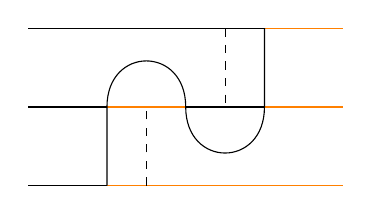
\begin{tikzpicture}
    \draw (0, 0)--(1, 0);
    \draw[orange] (1, 0)--(4, 0);
    \draw (0,1)--(1, 1);
    \draw[orange] (1, 1)--(2, 1);
    \draw (2, 1)--(3, 1);
    \draw[orange] (3, 1)--(4, 1);
    \draw (0, 2)--(3, 2);
    \draw[orange] (3, 2)--(4, 2);

    \draw (1, 0)--(1, 1) 
    to[out=90, in=90, looseness=2] (2, 1)
    to[out=-90, in=-90, looseness=2] (3, 1)
    to (3, 2);

    \draw[dashed] (1.5, 0) -- (1.5, 1);
    \draw[dashed] (2.5, 2) -- (2.5, 1);
  \end{tikzpicture}
\end{center}

zdjęcia + obrazki dla monady

maybe, reader monad
